% ARPEGOS:  Automatized Roleplaying-game Profile Extensible Generator Ontology based System %
% Author : Alejandro Muñoz Del Álamo %
% Copyright 2019 %

% Section 5.3: Diagrama de clases %
\section{Diseño de Implementación}
Después de realizar el diseño lógico de datos del sistema, el próximo paso es diseñar la estructura de clases del proyecto.
Esta estructura está compuesta por las diversas clases que se consideran necesarias para el funcionamiento de cualquier sistema 
orientado a objetos, y se puede representar mediante un \textit{diagrama de clases}, que muestra las clases de un sistema
con sus atributos y operaciones, y las relaciones entre éstas. A continuación se muestra el diagrama de clases del proyecto en 
la figura \ref*{DiagramaClases}.\medskip

\begin{figure}[ht]
    \centering
    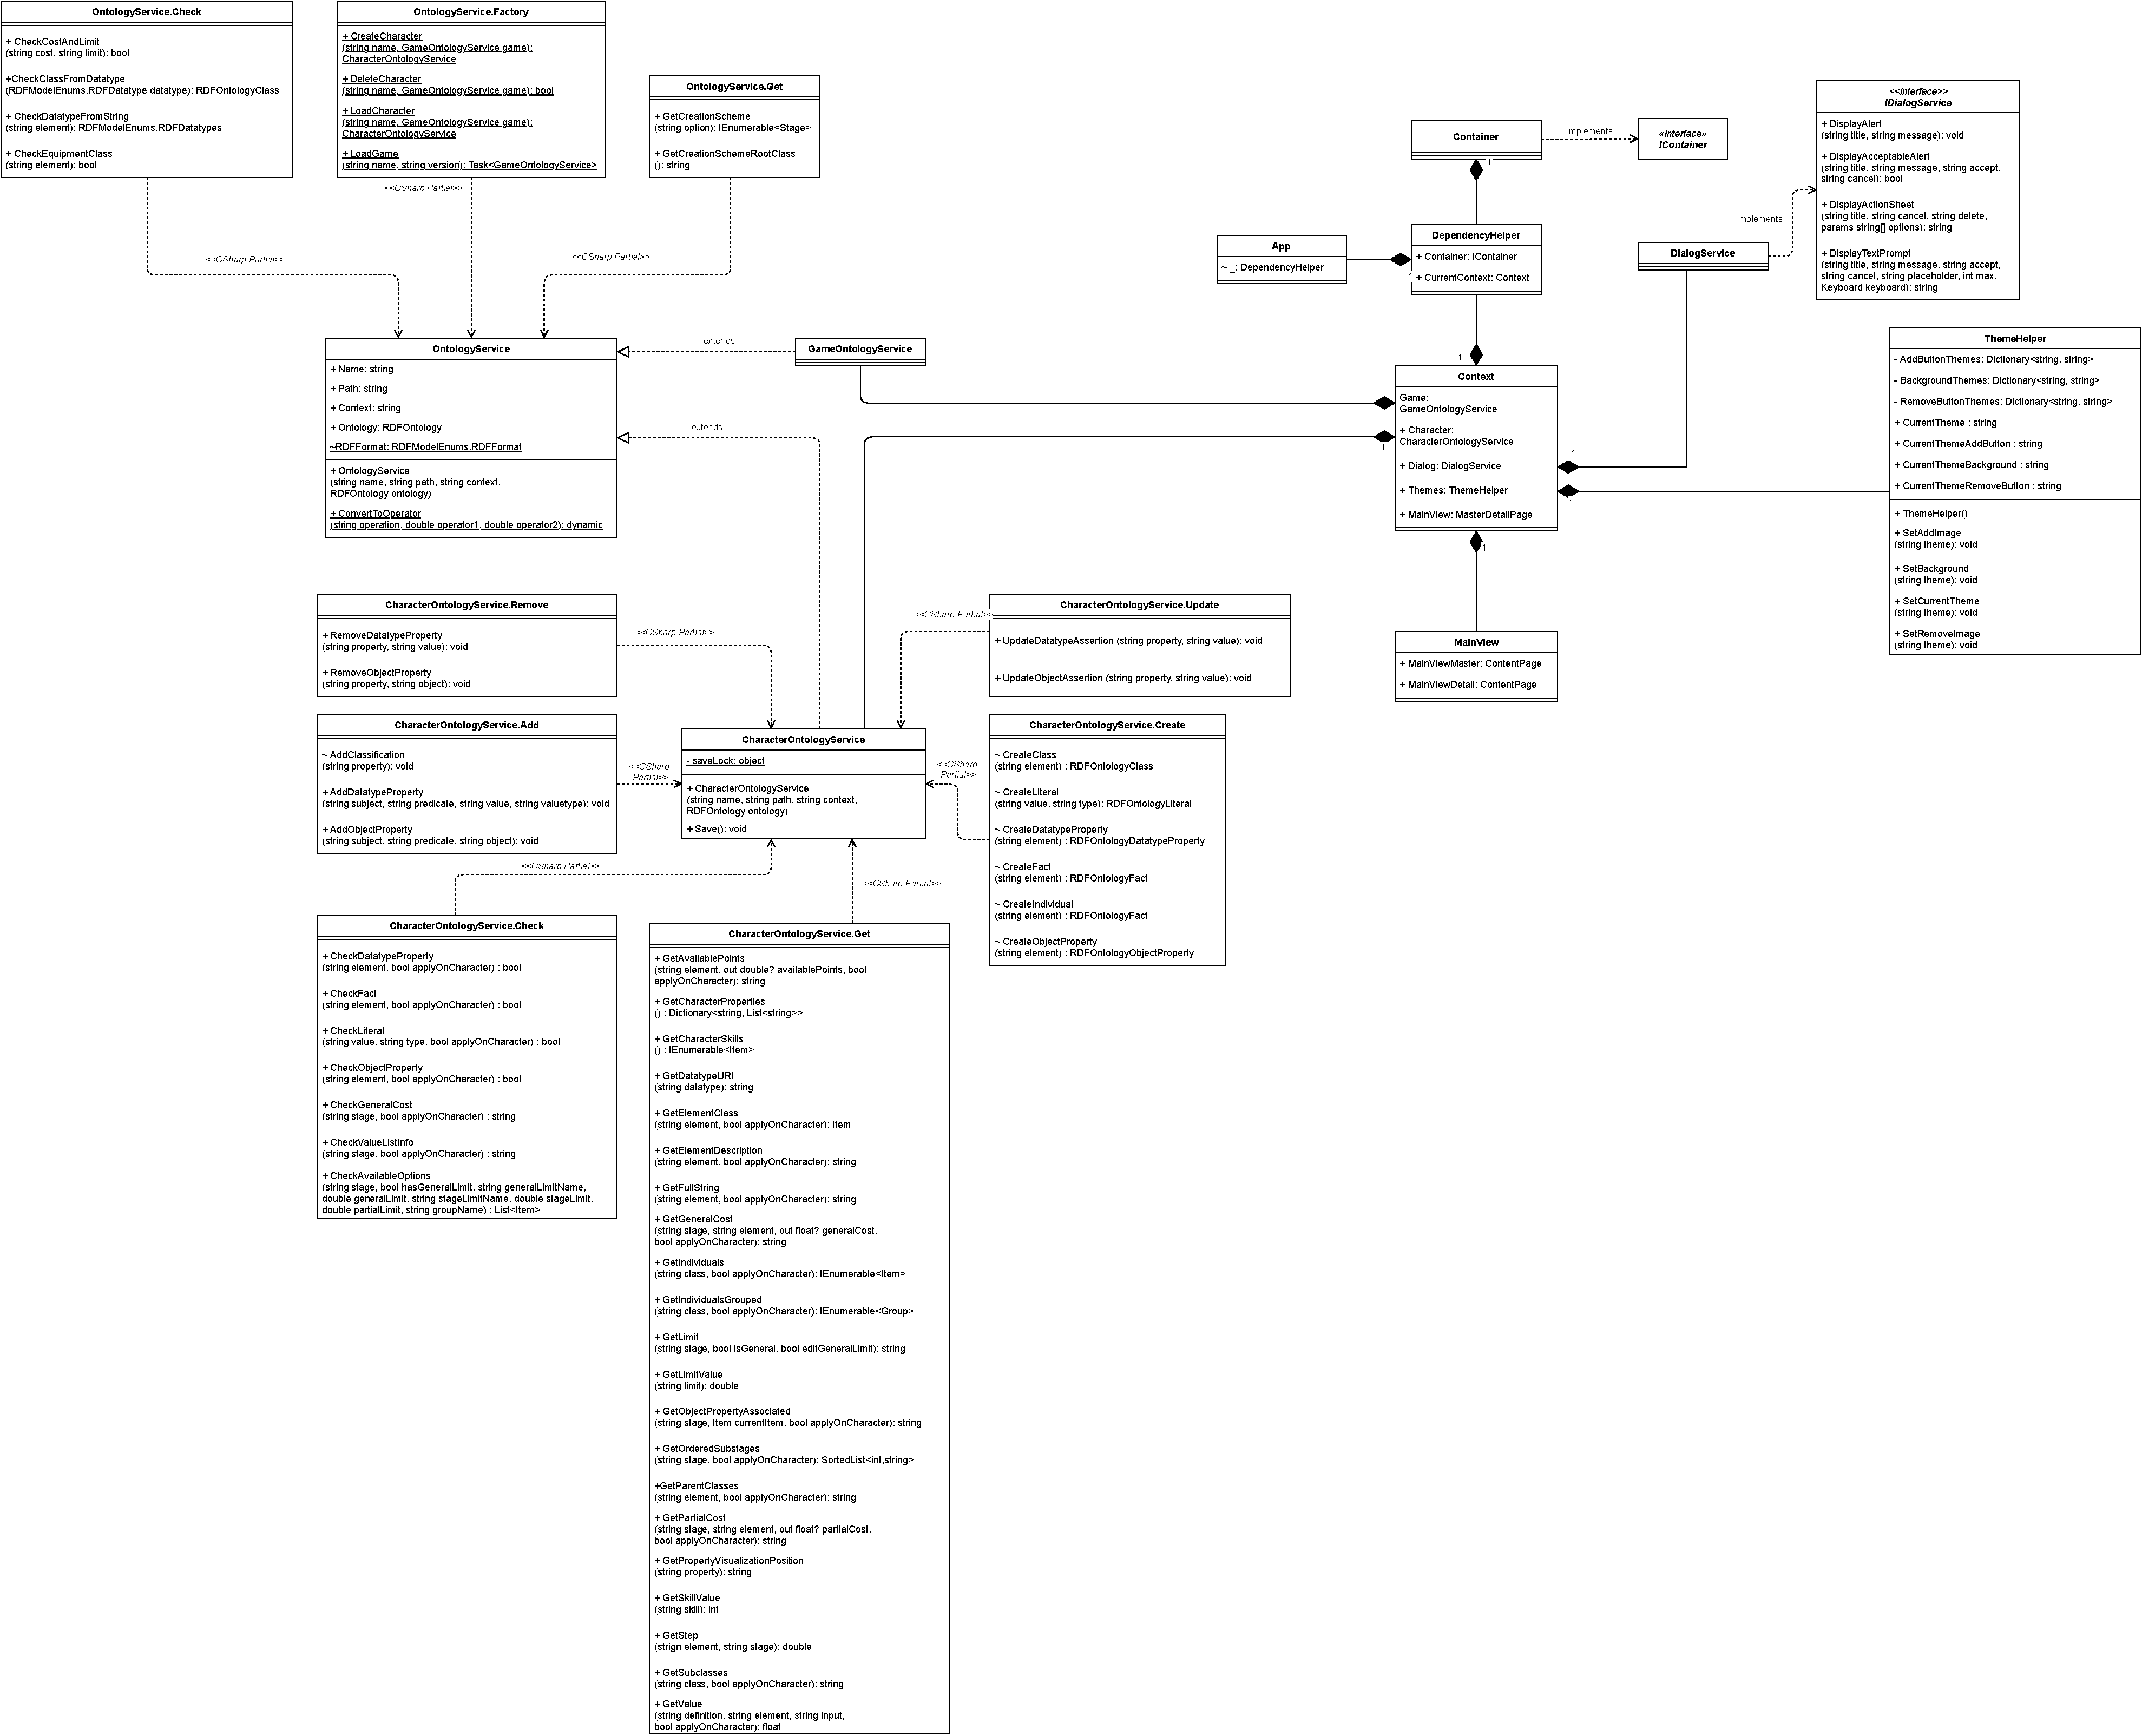
\includegraphics[scale=0.2]{Documentation-Scheme/Desarrollo/Diseño-Sistema/DiagramaClases.pdf}
    \caption{Diagrama de clases de \textit{ARPEGOS}}
    \label{DiagramaClases}
\end{figure}

Como se puede apreciar en el diagrama, algunas clases tienen una relación del tipo \textit{CSharp Partial}. 
Esta relación es una funcionalidad del lenguaje \textit{C\#} que permite implementar una misma clase en 
varios ficheros, lo que permite distribuir los atributos y métodos de una clase entre ellos para facilitar 
la legibilidad y mantenibilidad del código. Éstas clases parciales se pueden reconocer por contener el nombre 
de la clase con la que están relacionadas, seguidas de un punto y la primera palabra de los métodos que contienen.

\subsection{App}
Esta clase representa la aplicación en su conjunto. Contiene como atributo una instancia de la 
clase \textit{DependencyHelper}.

\subsection{DependencyHelper}
El \textit{DependencyHelper} contiene el contexto de la aplicación y los servicios y modelos de vista 
que muestran algún tipo de dependencia en el proyecto.

\subsection{Context}
La clase \textit{Context} dispone de varios elementos que pueden variar en base al funcionamiento de la 
aplicación. Estos elementos son: 
\begin{itemize}
    \item La ontología del juego actualmente seleccionado, de tipo \textit{GameOntologyService}.
    \item La ontología del personaje actualmente seleccionado, instancia de la clase \textit{CharacterOntologyService}.
    \item El servicio de temas de fondo, objeto de la clase \textit{ThemeHelper}.
    \item El servicio de pantallas de diálogo, de tipo \textit{DialogService};
    \item La vista principal de la aplicación, instancia de la clase \textit{MainView}.
\end{itemize}

\subsection{OntologyService}
El servicio \textit{OntologyService} modela cualquier ontología presente en el sistema del proyecto.

\subsection{GameOntologyService}
Esta clase describe la ontología de cualquier juego disponible en la aplicación, y como tal, 
hereda los atributos y métodos de la clase \textit{OntologyService}, sin añadir ninguna propiedad 
o función aparte de las ya heredadas. 

\subsection{CharacterOntologyService}
Esta clase, que es la más compleja del proyecto, dispone de todos los métodos necesarios para 
poder generar, modificar, actualizar y eliminar personajes de cualquier juego disponible en la aplicación. 

\subsection{ThemeHelper}
El servicio \textit{ThemeHelper} es aquel que dispone el tema de colores y fondo que se muestra 
en pantalla durante la ejecución de la aplicación.

\subsection{DialogService}
El servicio de diálogo permite mostrar ventanas emergentes según sean necesitadas durante la ejecución 
de la aplicación.

\subsection{MainView}
Esta clase modela la vista principal del proyecto. Está formada por dos vistas: la vista de detalles, 
que es la que está activa, y la vista maestra, que contiene el menú contextual.
